\documentclass{standalone}
\usepackage{tikz}
\usetikzlibrary{automata,calc,positioning,arrows}

\begin{document}
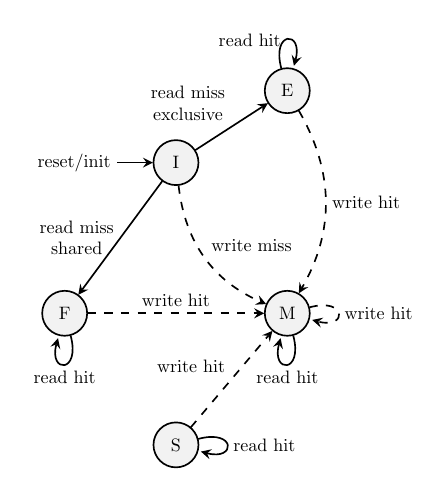
\begin{tikzpicture}[node distance=2.5cm,initial text={reset/init}]
	\tikzstyle{every node}=[scale=0.65]
	\tikzstyle{every state}=[semithick, fill=gray!10]
	\tikzstyle{every edge}=[draw,->,>=stealth,auto,semithick]

	\node[state, initial] (I) {I};
	\node[state,above right= 0.5cm and 1cm of I] (E) {E};
	\node[state,below right= 1.5cm and 1cm of I] (M) {M};
	\node[state,below= 3cm of I] (S) {S};
	\node[state,below left= 1.5cm and 1cm of I] (F) {F};

	\draw (M) edge[dashed,loop right] node[align=center] {write hit} (M)
	edge[loop below] node[align=center] {read hit} (M);
	\draw (S) edge[dashed] node[align=center] {write hit} (M)
	edge[loop right] node[align=center] {read hit} (S);
	\draw (E) edge[loop above] node[align=center,left] {read hit} (E)
	edge[dashed,bend left] node[align=center] {write hit} (M);
	\draw (F) edge[loop below] node[align=center] {read hit} (F)
	edge[dashed] node[align=center] {write hit} (M);
	\draw (I) edge[dashed,bend right] node[align=center] {write miss} (M)
	edge node[align=center] {read miss\\exclusive} (E)
	edge node[align=center,left] {read miss\\shared} (F);
\end{tikzpicture}
\end{document}
